\documentclass[12pt]{article}
\usepackage[spanish]{babel}
\usepackage[utf8]{inputenc}
\usepackage{csquotes}

% Interlineado 1.5
\usepackage{setspace}
\onehalfspacing

% Fuente Times New Roman
\usepackage{mathptmx}

% Acomodar margenes del documento
\usepackage[a4paper, margin=2cm, top=3cm, headheight=50pt]{geometry}

% Paquetes comunes
\usepackage{graphicx, float}
\usepackage{amsfonts, amssymb, amsmath}
\usepackage{physics, esvect}
\usepackage{enumerate}
\usepackage[colorlinks=true, citecolor=blue]{hyperref}

% Para graficar
\usepackage{pgfplots}
\usepackage{tikz, color}
\usepackage{tikz-3dplot}
\pgfplotsset{width=15cm, compat=1.12}

% Para automatas
\usetikzlibrary{automata, positioning, arrows, calc}
\tikzset{
        ->,  % makes the edges directed
        >=stealth, % makes the arrow heads bold
        shorten >=2pt, shorten <=2pt, % shorten the arrow
        node distance=3cm, % specifies the minimum distance between two nodes. Change if n
        every state/.style={draw=blue!55,very thick,fill=blue!20}, % sets the properties for each ’state’ n
        initial text=$ $, % sets the text that appears on the start arrow
}

% Encabezados
\usepackage{fancyhdr}
\pagestyle{fancy}
\fancyhf{}
\fancyfoot[C]{\thepage}
\fancyhead[L]{
  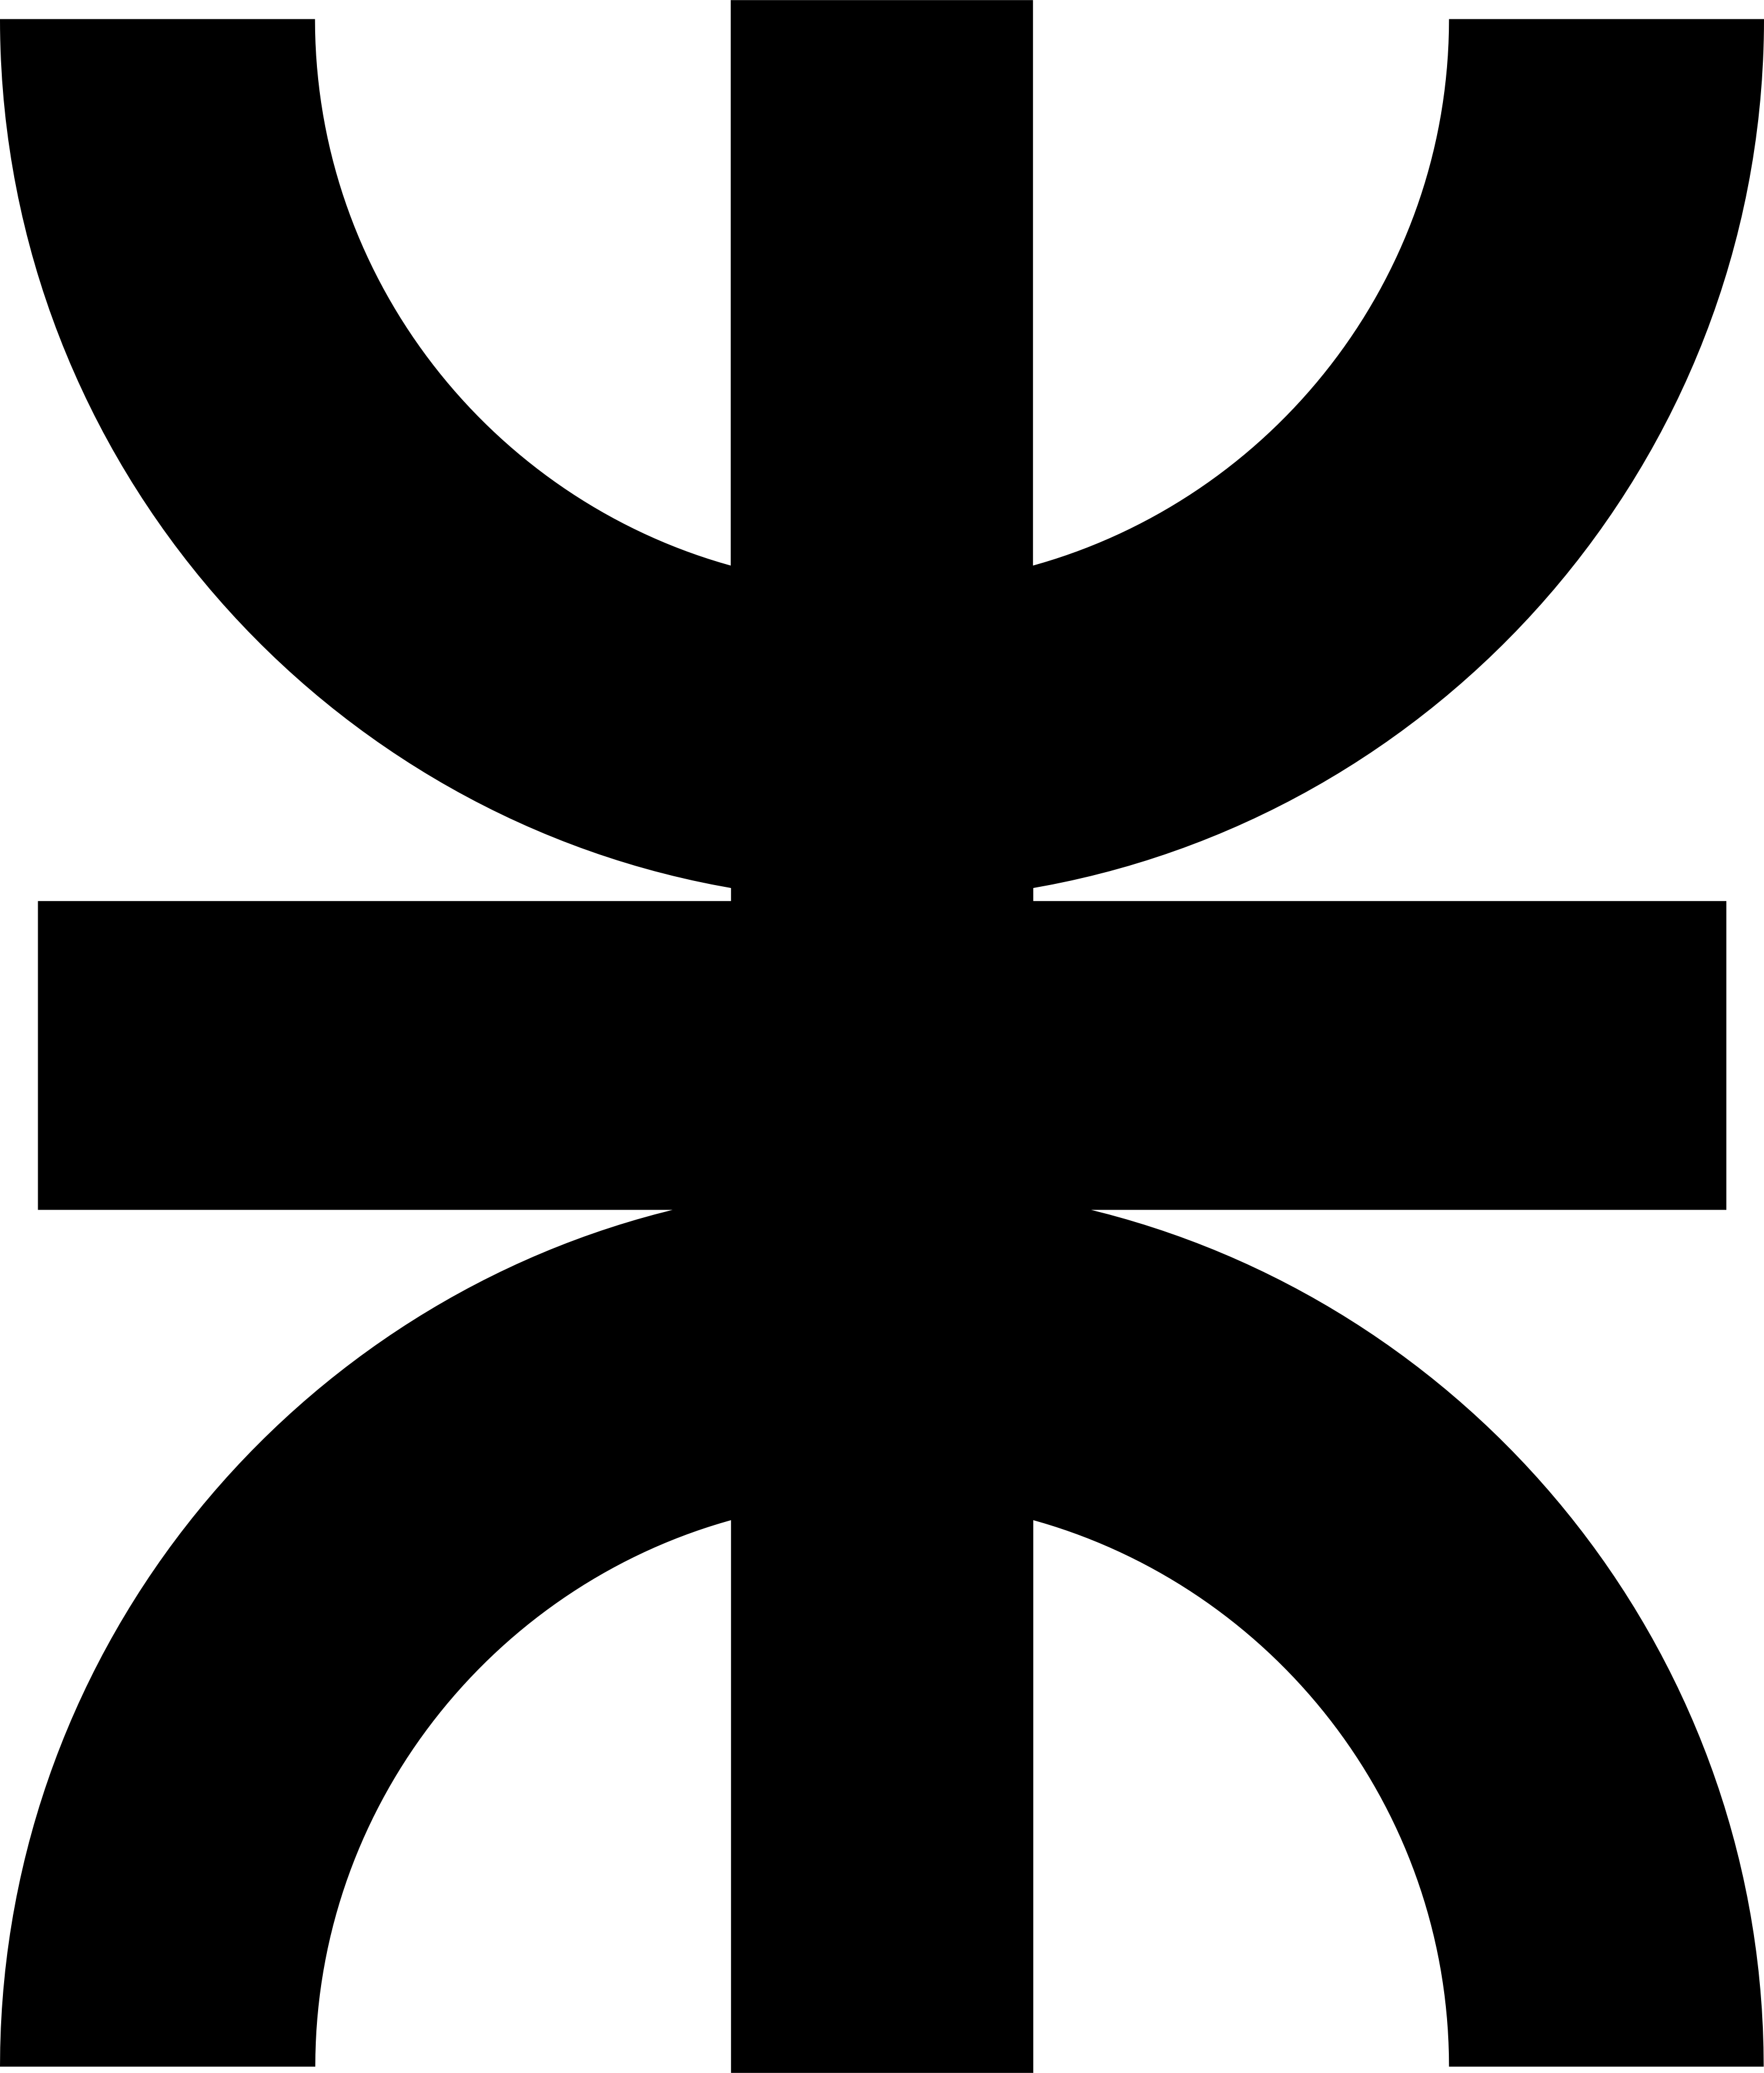
\includegraphics[height=1.2cm]{~/imagenes/logo_utn.png}
  \shortstack[l]{
    {\footnotesize Universidad Tecnológica Nacional} \\
    {\footnotesize Facultad Regional Córdoba} \\
    {\footnotesize Extensión Áulica Bariloche}
  }
}
\fancyhead[C]{
  \shortstack[c]{
    {\footnotesize Sistemas Operativos} \\
    {\footnotesize Resumen para el primer parcial} \\
    {\footnotesize }
  }
}
\fancyhead[R]{
  \shortstack[r]{
    {\footnotesize Profesor: Eduardo Tapia} \\
    {\footnotesize Alumno: Ricardo Nicolás Freccero} \\
    {\footnotesize Fecha: 24/05/2025}
  }
}

% Para bibliografía
\usepackage[backend=biber, style=apa]{biblatex}
\addbibresource{bibliografia.bib}

\begin{document}
\newgeometry{margin=2cm, top=1.5cm}
  \begin{titlepage}
    \centering
    
\includegraphics[width=\linewidth]{~/imagenes/logo_utn_frc.jpg}\\

    \textsc{
      \LARGE Universidad Tecnológica Nacional\\
      \Large Facultad Regional Córdoba - Extensión Áulica Bariloche\\
      \large Ingeniería en Sistemas de Información\\
      Año lectivo 2025\\[0.5cm]
    }

    \rule{\linewidth}{1.0mm}\\[0.4cm]
    \Huge
    \textbf{Sistemas Operativos}\\
    Resumen para el primer parcial\\[0.2cm]
    \LARGE
    Unidades 1, 2 y 3 de la cátedra
    \rule{\linewidth}{1.0mm}\\
    \large
    \begin{flushleft}
      Profesor: Eduardo Tapia

      Ayudante: 

      Fecha: 24/05/2025
    \end{flushleft}

    \vfill
    \begin{flushright}
      Alumno: Ricardo Nicolás Freccero

      Número de legajo: 415753
    \end{flushright}
  \end{titlepage}

  \restoregeometry
  \tableofcontents
  \newpage

  \section{Unidad 1 - Concepto de Sistemas Operativos}
  \subsection{¿Qué es el sistema operativo?}
  Un sistema operativo es un programa que controla la ejecución de aplicaciones y programas. Es quien se encarga de ``conectar'' o ``comunicar'' las apliaciones con el hardeware de la computadora. Se puede considerar que un sistema operativo tiene tres objetivos:

  \begin{itemize}
    \item \textbf{Facilidad de uso.} Un sistema operativo facilita el uso de un computador.

    \item \textbf{Eficiencia.} Un sistema operativo permite que los recursos de un sistema de computación se puedan utilizar de una manera eficiente.

    \item \textbf{Capacidad para evolucionar.} Un sistema operativo se debe construir de tal forma que se puedan desarrollar, probar e introducir nuevas funciones en el sistema sin interferir con su servicio.
  \end{itemize}

  \subsubsection{El sistema operativo como una interaz de usuario/computador}
  El hardware y software que le permiten al usuario acceder y utilizar las aplicaciones y programas de una computadora se pueden ver de forma jerárquica como muestra la Figura \ref{fig:jerarquia-sist-comp}. Al usuario no le suelen interesar los detalles del hardware de la computadora y vé al sistema de computación como un conjunto de aplicaciones. Por otro lado, cada aplicación se puede expresar en un lenguaje de programación y normalmente es desarrollada por un programador. Al programador sí le importan los detalles del hardware, pero no se comunica casi nunca directamente con él ya que suele ser una tarea extremadamente compleja. Para eso existe un \textit{conjunto de programas de sistema} que le permiten al programador comunicarse de una manera mas eficiente con el hardware. El programa de sistema mas importante es el \textbf{sistema operativo} que proporciona una interfáz entre el software y el hardware, actuando como mediador y facilitando el acceso del programador a las utilidades y servicios del sistema.

  \begin{figure}[H]
    \centering
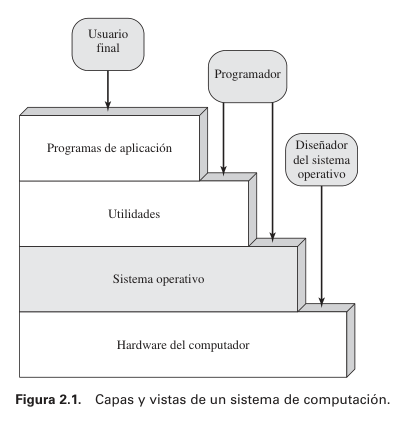
\includegraphics[width=0.4\linewidth]{imagenes/jerarquia-sist-comp.png}
    \caption{Imagen sacada de \parencite{sostallings}. Jerarquía de un sistema de computación.}
    \label{fig:jerarquia-sist-comp}
  \end{figure}

  El sistema operativo proporciona normalmente servicios en las siguientes áreas:
  \begin{itemize}
    \item \textbf{Desarrollo de programas.} Ofrece editores y depuradores para asistir al programador en la creación de programas y aplicaciones.

    \item \textbf{Ejecución de programas.} Se encarga de realizar todos los pasos necesarios para la ejecución de programas en nnombre del usuario.

    \item \textbf{Acceso a dispositivos de E/S.} Facilita el acceso de los programadores a estos dispositivos.

    \item \textbf{Acceso al sistema.} Protege los recursos y los datos,e vitando el uso no autorizado de los ususarios y resolviendo conflictos en el caso de conflico de recursos.

    \item \textbf{Detección y respuesta a errores.} Debe proporcionar una respuesta a cualquier error que pueda surgir de manera que se elimine la condición de error, suponiendo el menor impacto en las aplicaciones que están en ejecución. 

    \item \textbf{Contabilidad.} Recoge estadísticas de uso de los diferentes recursos y monitoriza parámetros de rendimiento. Esta información es útil para anticipar las necesidades de mejoras futuras y para optimizar el sistema a fin de mejorar su rendimiento.
  \end{itemize}

  \subsubsection{El sistema operativo como gestor de recursos}
  El sistema operativo dirige al procesador en el uso de los recursos de la computadora y en el tiempo que debe tomarse para la ejecución de otros programas. Para eso, el sistema operativo cede el control para que el procesador realice sus tareas y luego retoma el control para decirle qué sigue.

  El sistema operativo decide cuándo un programa en ejecución puede utilizar un dispositivo de E/S y controla el acceso y uso de los ficheros, además decide cuánto tiempo debe tomarse cada procesador para la ejecución de un programa.

  \subsubsection{Facilidad de evolución de un sistema operativo}
  Un sistema operativo debe evolucionar en el tiempo por las siguientes razones:
  \begin{itemize}
    \item Actualizacioes de hardware y nuevos tipos de hardware.

    \item Nuevos servicios. (Por ejemplo, si es dificil mantener un buen rendimiento con las herramientas existentes, se pueden añadir al sistema operativo nuevas herramientas de medida y control.)

    \item Resolución de fallos.
  \end{itemize}

  \subsection{Evolución de los sistemas operativos}
  \subsubsection{Procesamiento en serie}
  El programador interactuaba directamente con el hardware de la computadora, que contaba con una consola, luces, interruptores, algún dispositivo de entrada y una impresora; \textit{no existía ningún sistema operativo}. Los programas en código máquina se cargaban a través del dispositivo de entrada y si un error provocaba la parada del programa, las luces indicaban la condición de error. El programador podía examinar los registros del procesador y memoria principal para determinarl la causa del error. Si el programa terminaba de forma normal, la salida se imprimía.

  \subsubsection{Sistemas en lotes sencillos}
  Se empieza a usar un software denominado \textbf{monitor}, que permite que el usuario no tenga que acceder directamente a la máquina. En su lugar, el la computadora recibe una secuencia de trabajos que va a usar el monitor. El monitor de encarga de leer uno a uno cada trabajo y decirle al procesador que los vaya realizando en ese orden.

  \subsubsection{Sistemas en lotes multiprogramados}
  Aún usando un sistema de lotes sencillos, el procesador está haciendo nada la mayoría del tiempo ya que este es mucho mas rápido que los dispositivos de E/S. La computadora pasa mas tiempo buscando la información que tiene que procesar el procesador que procesando esa información. Lo que se puede hacer entonces es que mientras se está esperando por la E/S, se le puede asignar al procesador otro trabajo que no esté esperando por una operación de E/S. 

  \begin{figure}[H]
    \centering
    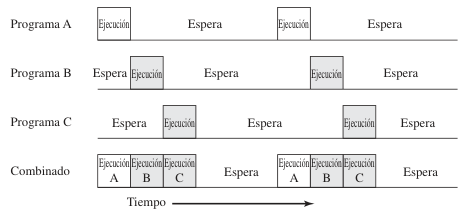
\includegraphics[width=0.5\linewidth]{imagenes/multiprogramacion.png}
    \caption{Imagen sacada de \parencite{sostallings}. Ejemplo de multiprogramación con tres programas.}
    \label{fig:multiprog}
  \end{figure}
  

  \subsubsection{Sistemas de tiempo compartido}
  Son sistemas que comparten el tiempo de programación entre múltiples usuarios.

  \subsection{Desarrollos que llevaron a los sistemas operativos modernos}
  \subsubsection{Arquitectura micronúcleo o microkernel}
  Antes, la mayoría de los sistemas operativos estaban formados por \textbf{núcleos monolíticos}. Estos núcleos proporcinaban la mayoría de las funcionalidades consideradas propias del sistema operativo, incluyendo planificación, los sistemas de ficheros, las redes, los controladores de dispositivos, la gestióno de memoria, etc. Una \textbf{arquitectura microkernel} asigna sólo unas pocas funciones esenciales al kernel, incluyendo los espacios de almacenamiento, comunicación entre procesos, y planificación básica.

  \subsubsection{Multithreading}
  Es una técnica en la cual un proceso, ejecutando una aplicación, se divide en una serie de \textit{hilos} o \textit{threads}.
  \begin{itemize}
    \item \textbf{Thread o hilo.} Es una unidad de trabajo. Incluye el contexto del procesador (que contiene el contador del programa y el puntero de pila) y su propia área de datos para una pila (para posibilitar el salto a subrutinas). Un hilo se ejecuta secuencialmente y se puede interrumpir para dar paso a otro hilo.

    \item \textbf{Proceso.} Es una colección de uno o más hilos y sus recursos de sistema asociados. Es un programa en ejecución.
  \end{itemize}

  Esta técnica es útil para aplicaciones que llevan a cabo tareas que no necesitan correrse en serie, es decir, que se pueden ejecutar en simultáneo.

  \subsubsection{Multiprocesamiento simétrico (SMP)}
  Se refiere a la arquitectura del hardware de la computadora y al comportamiento del sistema operativo que explota dicha arquitectura. Tiene las siguientes características:
  \begin{itemize}
    \item Tiene múltiples procesadores.

    \item Los procosadores comparten las mismas utilidades de momeira principal y de E/S.

    \item Todos los procesadores pueden realizar las mismas funciones.
  \end{itemize}

  El sistema operativo de un SMP planifica procesos o hilos a través de todos los procesadores.
  \begin{figure}[H]
    \centering
    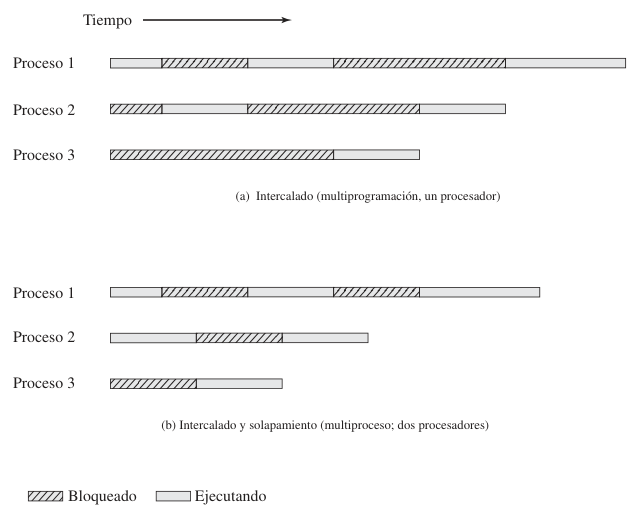
\includegraphics[width=0.7\linewidth]{imagenes/smp-vs-no-smp.png}
    \caption{Imagen sacada de \parencite{sostallings}. Multiprogramación y multiproceso.}
    \label{fig:smp}
  \end{figure}
  
  \subsubsection{Sistema operativo distribuído}
  Da la ilusión de tener un solo espacio de memoria principal y un solo espacio de memoria secundario, cuando tenemos un ``cluster'' de computadoras (varias computadoras que operan como si fuese una sola).

  \subsubsection{Diseño orientado a objetos}
  Introduce una disciplina al proceso de añadir extensiones modulares a un pequeño núcleo. Permite a los programadores personalizar un sistema operativo sin eliminar la integridad del sistema.

  \subsection{Sistemas UNIX tradicionales}
  UNIX es un sistema operativo que se desarrollo inicialmente en los laboratorios de Bell y se hizo operacional en 1970. En la figura \ref{fig:arq-unix} se puede ver la arquitectura general de UNIX.

  \begin{figure}[H]
    \centering
    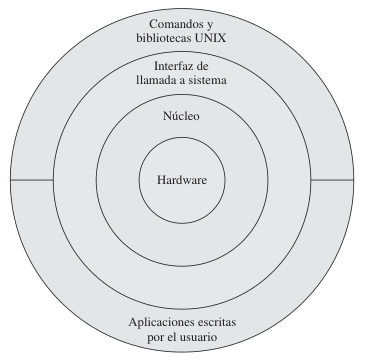
\includegraphics[width=0.6\linewidth]{imagenes/arquitectura-unix.png}
    \caption{Imagen sacad de \parencite{sostallings}. Arquitectura general de UNIX.}
    \label{fig:arq-unix}
  \end{figure}

  \subsection{Linux}
  Linux comenzó como una variante UNIX. Linus Torvalds, un estudiante finlandés de informática, escribió la versión inicial. Linux es un sistema UNIX completo de software libre (cualquier persona puede ver y modificar el código fuente).

  La mayoría de los núcleos de Linux son monolíticos.  Aunque no usa la técnica de microkernel, logra muchas de las ventajas potenciales de esta por medio de su arquitectura modular particular. Linux está estructurado como una colección de módulos, algunos de los cuales pueden cargarse y descargarse automáticamente bajo demanda. Estos bloques se denominan \textbf{módulos cargables}.

  Los módulos cargables de Linux tienen dos características importantes:
  \begin{itemize}
    \item \textbf{Enlace dinámico}. Un módulo de núcleo puede cargarse y enlazarase al núcleo mientras el núcleo está en memoria y ejecutándose. Un módulo también puede desenlazarase y eliminarse de la memoria en cualquier momento.

    \item \textbf{Módulos apilables}. Los módulos se gestionan como una jerarquía. Cuando un módulo superior en la jerarquía referencia a un módulo inferior, el primero actúa como módulo cliente y el segundo como biblioteca.
  \end{itemize}

  \section{Unidad 2 - Administración y Gestión de Archivos}
  Los \textbf{archivos} son unidades logicas de informacion que pueden ser leidas o creadas por los procesos. La informacion que se almacena en los archivos debe ser persistente. Un archivo debe desaparecer solo cuando su propietario lo remueve de manera explicita.

  Los archivos son administrados por el sistema operativo. La parte del sistema operativo que trata con los archivos se conoce como \textbf{sistema de archivos}.

  \subsection{Archivos}
  Los archivos proporcionan una manera de almacenar informacion en el disco y leerla despues. Cuando un proceso crea un archivo le proporciona un nombre. Cuando el proceso termina, el archivo sigue existiendo y puede ser utilizado por otros procesos mediante su nombre.

  Algunos sistemas de archivos, como el de UNIX, diferencian las letras mayusculas de las minusculas, mientras que otros no.

  Existen varios sistemas de archivos que vamos a analizar mas adelante. Por ahora solo vamos a decir que Windows 95 y 98 usan el sistema de archivos \textbf{FAT-16}. Windows 98 extendio FAT-16 e introdujo \textbf{FAT-32} pero estos dos sistemas son bastante similares. Las versiones mas nuevas de Windows admiten ambos sistemas FAT, que en realidad ya son obsoletos, pero tienen un sistema de archivos nativo que se conoce como \textbf{NTFS}.

  Muchos sistemas operativos aceptan nombres de archivos en dos partes, separadas por un punto. La parte que va despues del punto se conoce como la \textbf{extension del archivo} y suele indicar algo acerca de la naturaleza de ese archivo.
  
  En algunos sistemas (como UNIX) las extensiones de archivo son solo convenciones y no son impuestas por el sistema operativo. Funcionan mas como un recordatorio para el propietario que como un medio para transportar informacion a la computadora. Sin embargo, en otros sistemas (como Windows) 'este es consciente de las extensiones y les asigna significado. Los usuarios pueden registrar extensiones y asignar programas a cada una de manera que cuando se le hace doble click al nombre del archivo, el programa asignado a su extension se inicia con ese archivo como parametro.

  \subsection{Estructura de archivos}
  Los archivos se pueden estructurar de varias formas:
  \begin{itemize}
    \item \textbf{Secuencias de byte sin estructura.} El sistema operativo no sabe, ni le importa que hay en el archivo. Esto provee la maxima flexibilidad ya que los programas de usuario pueden colocar cualquier cosa que quieran en sus archivos y denominarlos de cualquier manera conveniente.

    \item \textbf{Secuencia de registros.} Un archivo es una secuencia de registros de longitud fija, cada uno con cierta estructura interna. Estos sistemas se usaban cuando todavia se utilizaban las tarjetas perforadas de 80 columnas, de manera que cada registro consistia de 80 caracteres, simulando la tarjeta.

    \item \textbf{Arbol.} Un archivo consiste en un arbol de registros, donde no todos son necesariamente de la misma longitud; cada uno de llos contiene un campo llave en una posicion fija dentro del registro. El arbol se ordena con base en el campo llave para permitir una busqueda rapida por una llave especifica.
  \end{itemize} 

  poner figura 4-2 pagina 289 tannenbaum

  \subsection{Tipos de archivos}

  


  

  \newpage
  \addcontentsline{toc}{section}{Referencias}
  \printbibliography

\end{document}
